% !TeX program = xelatex
% DRAFT generated 2026-10-15 from the zero-cost analyses in this repository.
% Part A numbers are real (reports/data/*.json, papers/search/*.csv). \tbd{} marks Part B placeholders.
\documentclass[11pt,a4paper]{article}
\usepackage{aes}
\usepackage{amsmath,tabularx,booktabs,xcolor}
\newcommand{\tbd}[1]{\textcolor{red}{[#1]}}

\title[What Does a MemoryAgentBench Score Measure?]{What Does a MemoryAgentBench Score Measure?\\A Harness and Claims Audit of an Agent-Memory Leaderboard}
\aesauthor[affil={1},corresponding]{Eric Sun}
\aesaffiliation{1}{\tbd{Affiliation}}
\aesemails{\aesemail{\tbd{email}}}
\aeskeywords{Agent memory; Benchmark reliability; Replication; Measurement validity}

\begin{document}
\maketitle

\begin{abstract}
MemoryAgentBench (MAB) has become a de facto leaderboard for agent memory. In the 15 months after its release,
41 papers, pull requests and issues reported their own MAB numbers. We ask what a MAB score can support. First, an
offline audit of the public evaluation harness finds that Mem0 stores memories under one key and queries
another, so it answers without its own memory. We verify this by running the vendored Mem0 with stubbed models.
Cognee and Zep are mis-isolated in related ways (shown in stubbed execution and code reading), and RAG agents
with smaller input limits silently drop the oldest history. \tbd{Effect: fixed Mem0 scores $a$ vs.\ $b$ under the
public harness and $c$ closed-book.} On LongMemEval(S*) the original paper's Mem0 score exceeds its long-context backbone (36.0 vs.\ 30.7), so the
original runs probably used working code; the risk lies with later re-runs through the public harness. Second, from these sources we extract 268
quantitative comparisons; a hand check of 30 found every score correct, though 6 of 30 had wrong metadata flags.
Of 147 claimed improvements from 29 sources, 37--48\% fall within the item-sampling noise of the benchmark's
question sets (paired vs.\ unpaired bounds), mostly in per-split comparisons. Each source's headline claim is
within noise for only 9 of 29 sources. Only 9 of the 29 sources report any uncertainty, and 12 of 144 cells in
MAB's own tables changed between paper versions without a changelog. The long-context vs.\ BM25 findings and most headline averages survive item noise. A large share of per-split comparisons, and conclusions drawn from
re-run memory-system baselines, need re-examination. We release offline check scripts, the audited claims and a
minimal reporting protocol.
\end{abstract}

\section{Introduction}
\label{sec:intro}
Memory benchmarks for LLM agents feed questions to a system after streaming it a long history, and they score
the answers. MemoryAgentBench \citep{hu2026memoryagentbench} reformulates long-context datasets into incremental
multi-turn streams. It covers four competencies (accurate retrieval, test-time learning, long-range
understanding, conflict resolution) and evaluates long-context models, RAG pipelines and agentic memory systems
side by side. Within a year it has become a leaderboard. New memory systems report MAB numbers next to baselines
copied from the original paper, and vendors add their methods to its repository.

Several properties of MAB make a single score fragile. Most splits contain about 100 questions that share
\emph{one} context and therefore one memory build. Systems are run once, in one ingestion order, with one prompt
template. Some systems (e.g.\ Mem0) build their memory with an LLM at nonzero temperature, so the memory itself is
a random variable, yet it is built once. None of this is unusual. Single runs remain the norm in memory
evaluation, and run-to-run variance, judge sensitivity and confounds have now been documented for other memory
benchmarks \citep{chanhnourack2026auditing,mishra2026merit,spencer2026groundtruth,wang2026memdelta,jung2026meme}.
What is missing is an account of which comparisons on the benchmark people actually use are resolvable.

\paragraph{Contributions.} (0) An offline audit of the public MAB harness, including a keying bug that disconnects Mem0 from its
memories at question time (Section~\ref{sec:harness}). (1) An audit of 147 published improvements on MAB against item-sampling noise, with
per-claim matching to the split and number of questions (Section~\ref{sec:audit}). (2) Evidence that published
numbers drift. MAB's own tables change between versions without a changelog, and independent reproductions of
LLM-built memory systems miss by a median of 9.2 points (Section~\ref{sec:drift}). (3) A three-arm check of Mem0 (public harness, fixed, closed-book) that turns the harness finding into an effect
size \tbd{results}; optionally, a rebuild~$\times$~order~$\times$~item experiment (Section~\ref{sec:partb}). (4) A reporting protocol (Section~\ref{sec:protocol}).

\section{Harness integrity: memory systems without their memory}
\label{sec:harness}
In the public harness (from the initial public commit of 5 July 2025, two days before the first arXiv version, through the current main branch), \texttt{initialization.\_memorize\_context\_chunks}
calls \texttt{send\_message(chunk, memorizing=True)} without a context identifier, so it defaults to
\texttt{None}. Queries are sent with \texttt{context\_id} set to the context index. Mem0 keys memories by
\texttt{user\_id=context\_\{context\_id\}\_\{dataset\}}, Cognee by a dataset name and Zep by a graph id
built the same way. Writes therefore go to \texttt{context\_None\_*} and reads to \texttt{context\_0\_*}.
We confirmed this without any API calls. With the real vendored Mem0 and its local vector store, stubbing only
the LLM and embedder, the public path stores memories under \texttt{context\_None\_*} and retrieves none for
\texttt{context\_0\_*}; passing the identifier retrieves them all. A recorder version of the same check drives
the unmodified harness path. Every \texttt{add} used \texttt{context\_None\_factconsolidation\_sh\_6k}, the \texttt{search}
used \texttt{context\_0\_factconsolidation\_sh\_6k}, and zero memories were retrieved. Cognee's vendored search ignores the dataset key, so the keying is moot, but a query on context $i$ searches every
context memorized so far, $0..i$ (cross-book leakage on multi-context splits; shown with stubbed execution). Zep reads a
graph that is never created (code reading; whether the run crashes or receives empty context is untested). Long-context and
RAG agents and the community-added memory methods do not key on this identifier. The same audit finds that RAG
agents with 250--300K input limits silently drop the oldest chunks (keeping 56--65\% of RULER-QA2), that exact
match on DetectiveQA and the classification sets rejects the output formats the prompts request, and that every
released configuration sets the answer temperature to 0.7 (a few systems override it). The
issue tracker records the symptom (``memory is often empty'') but attributes it to the memory systems themselves.
\tbd{Effect size: Mem0 fixed vs.\ buggy on FactConsolidation, EventQA and LongMemEval(S*).} We cannot tell
whether the published numbers were produced with this code path, and there is evidence they were not. The
published Mem0 score on LongMemEval(S*) (36.0) exceeds its own long-context backbone (30.7), which is hard to
reach with an empty memory. Our claim therefore concerns the \emph{public} harness that later work uses for
reproductions and new baselines. An independent run of the official
configuration reproduced 15.3 against the published 36.0 for Mem0 on LongMemEval(S*).

Table~\ref{tab:harness} summarises all findings.

\begin{table}[t]
\centering\footnotesize
\begin{tabularx}{\linewidth}{@{}l X p{2.2cm} p{2.0cm} p{2.0cm}@{}}
\toprule
ID & Finding (public harness, commit 5380260) & Affects & Effect & Evidence \\
\midrule
A1 & Mem0 memorizes under context\_None, searches context\_i $\rightarrow$ retrieves nothing & Mem0 & no retrieval & executed (real Mem0) \\
A2 & Cognee search ignores dataset key $\rightarrow$ a query on context i also searches earlier contexts (0..i) & Cognee & cross-context leakage & stubbed execution \\
A3 & Zep reads a graph that was never created (graph\_None written, graph\_0 read) & Zep & likely crash / empty & code reading \\
B1 & RAG chunk store silently drops oldest chunks above 250--300K tokens & 4 systems & evidence lost & measured \\
B2 & Long-context truncation keeps only the tail (128K models keep 8--61\% of long main-tier contexts) & LC (GPT-4o-mini) & evidence lost & measured \\
B3 & Zep ingests only the first 9,998 chars of each chunk (~50--63\% stored) & Zep & evidence lost & code + measured \\
B4 & Retrieval/reader settings differ from configs (RAPTOR k=4 not 10; HippoRAG reader sees 5 of 10; fixed readers) & RAPTOR, HippoRAG-v2, Self-RAG & fewer passages & code reading \\
C1 & DetQA exact match $\approx$0 for answers in the prompted JSON format; 5/71 gold malformed & 14 systems & false negatives & offline run \\
C2 & ICL exact match rejects the instructed 'label: N' format & 14 systems & false negatives & code + README \\
C3 & Substring match credits hedged FC answers and 'I don't know' vs gold 'no' (12/100 RULER-QA2); some systems have no output cap & 7 systems & false positives & code reading \\
D1 & All 32 configs set temperature 0.7 (a few systems override it); scores are single runs & 13 systems & unreported variance & configs (32/32) \\
E1 & LongMemEval judge uses unpinned gpt-4o; stale verdicts reused & 14 systems & judge drift & code reading \\
\bottomrule
\end{tabularx}
\caption{Harness findings by effect and strength of evidence. Effects on the \emph{published} MAB numbers are not established: the original runs may have used different code (Section~\ref{sec:harness}).}
\label{tab:harness}
\end{table}


\paragraph{Exposure of published claims.} Of the 268 audited comparisons, 15 (from 8 sources) use Mem0, Cognee or
Zep as the baseline, and 12 of these (6 sources) re-ran that baseline themselves, and 10 of those 12 report gaps under 3 points. If those
re-runs went through the public harness, they inherit the defects above. The sources do not say which code path they used.

\paragraph{Not specific to MAB.} The same offline reading of other widely used memory-evaluation code finds related
defects. In the last released version of Mem0's LoCoMo evaluation, the Zep baseline ingests only the first of ten
conversations (\texttt{if idx == 0}) but is queried on all ten. In LoCoMo, 444 of 1{,}986 questions (22.4\%), all
of them adversarial (444 of 446 in category 5), lack an answer field, consistent with \citet{tanguturi2026atant}. Truncation keeps the newest history in
MAB's long-context agents but the oldest in LoCoMo and LongMemEval baselines.

\section{Part A: What the published numbers support}
\label{sec:audit}
\paragraph{Benchmark structure.} We computed split sizes from the released data. Each FactConsolidation
length, each in-context-learning set and each RULER-QA split has a single context with 100 questions. EventQA
has 5 books $\times$ 100 questions per length variant and is 6-way multiple choice (chance 16.7\%). DetectiveQA
has 71 four-way multiple-choice questions (chance 25\%). The harness takes the first $N$ items
deterministically. Every released agent configuration sets temperature 0.7, and Mem0 runs its extraction
at temperature 0.1, once per context. Yet each score comes from a single run.

\paragraph{Re-reading the original results.} Treating each cell of MAB's main table as a proportion over its
questions and resampling 4{,}000 times, the overall ranking is fairly stable: median Kendall $\tau=0.94$. The
probability of reproducing the top three, however, is only 86\%, falling to 61\% under a design effect of 4 that
stands in for clustering and run variance. In every column, 19--21 of the 21 adjacent pairs are within 95\% item
noise. Two headline findings survive item noise with $P\ge0.89$ even at a design effect of 4: BM25 retrieval beats its
GPT-4o-mini long-context backbone on accurate retrieval ($+11.3$), and long context beats BM25 on long-range
understanding ($+10.6$). Mem0's deficit to its backbone ($-21.1$ overall) is statistically robust too, but
Section~\ref{sec:harness} shows why memory-system numbers need a separate validity check. Fine-grained orderings do
not survive: Mem0 vs.\ Cognee ($+0.5$), HippoRAG-v2 vs.\ BM25 ($+0.1$), Claude-3.7 vs.\ GPT-4o ($+0.8$), and the
embedding models. On DetectiveQA, Zep (28.2) and Cognee (29.6) are not distinguishable from guessing ($n=71$,
one-sided binomial $p=0.31$ and $0.22$). Appendix Figure~\ref{fig:ranks} shows the rank uncertainty.

\paragraph{Claims audit.} We collected every source that reports its own numbers on any MAB split: 36 arXiv
papers plus GitHub pull requests and issues, from July 2025 to October 2026. From these we extracted 268
quantitative comparisons with scores, baseline, $n$, provenance of the baseline (re-run vs.\ copied), number of
runs and any uncertainty reported. Independent verification of a random 30-row sample found all 60 scores
correct. Six of the 30 rows had a wrong uncertainty or copied-baseline flag, and three rows from one source compared averages over four lengths with single-length baselines. Both systems in a claim are scored on the same first-$N$ items, so the appropriate test is paired, but no source
releases per-item outputs. We therefore bracket the answer. A paired test that assumes the discordant fraction is
$|\Delta|+10$ points (an optimistic, low-discordance assumption) finds 37\% of the 147 claimed improvements
within 95\% noise. An unpaired test, $z=\Delta/\sqrt{p_1q_1/n+p_2q_2/n}$, finds 48\%. Both ignore the
clustering of questions on one context, reruns, rebuilds and version drift, which all widen intervals. Under
either test, 96\% (paired: 90\%) of claims with gaps under 5 points are within noise, as are 54\% (43\%) of
claims labelled state of the art. The median claimed gap is 8 points (Figure~\ref{fig:claims}). Only 9 of the 29 sources (11 of all 41) report any uncertainty on MAB numbers. Counting claims per source does not drive the result. The source-weighted fraction within noise is 54\%, and
drawing one random claim per source gives 54\% (90\% range 41--66\%). Each source's \emph{headline} claim
(its largest-$n$ state-of-the-art comparison, or its largest-$n$ claim if it makes none; often an average over many splits) is within noise for only 9 of
29 sources. Aggregate headline claims are therefore mostly resolvable, while the per-split comparisons used to
argue for specific mechanisms often are not.

Table~\ref{tab:mdd} gives each split's resolution limit: on the 100-question splits, two single runs must differ by
about 9--20 points before a difference is reliably detectable.

\begin{table}[t]\centering\footnotesize
\begin{tabular}{@{}lrrrrr@{}}\toprule
Split & $n$ & contexts & MDD$_{95}$ & MDD$_{80}$ & MDD$_{80}$ paired \\\midrule
FactConsolidation (each length) & 100 & 1 & 13.9 & 19.8 & 8.9--12.5 \\
RULER-QA1 / QA2 & 100 & 1 & 13.9 & 19.8 & 8.9--12.5 \\
ICL (each set) & 100 & 1 & 13.9 & 19.8 & 8.9--12.5 \\
DetectiveQA & 71 & 10 & 16.4 & 23.5 & 10.5--14.9 \\
InfBench-Sum & 100 & 100 & 13.9 & 19.8 & 8.9--12.5 \\
Recsys & 200 & 1 & 9.8 & 14.0 & 6.3--8.9 \\
LME(S*) & 300 & 5 & 8.0 & 11.4 & 5.1--7.2 \\
EventQA (one length) & 500 & 5 & 6.2 & 8.9 & 4.0--5.6 \\
\bottomrule\end{tabular}
\caption{Smallest accuracy gap (points) that MAB splits can resolve between two single runs at $p=0.5$: MDD$_{95}$ is significant half the time; MDD$_{80}$ gives 80\% power. The paired column assumes 10--20\% discordant items. Binomial approximation (InfBench-Sum and Recsys are graded metrics); clustering on few contexts makes all of these optimistic.}
\label{tab:mdd}
\end{table}


\begin{figure}[t]
\centering
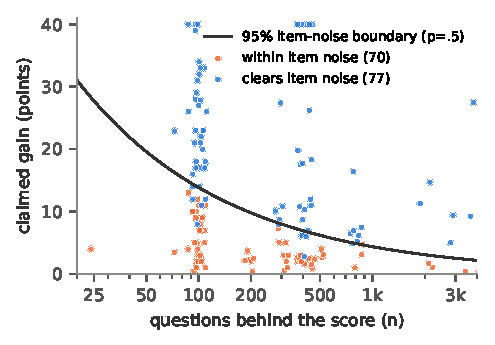
\includegraphics[width=0.49\linewidth]{figs/fig_claims.pdf}\hfill
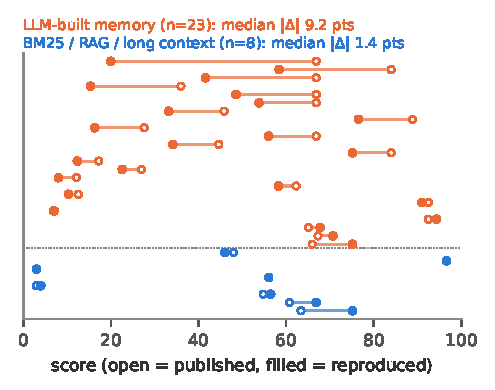
\includegraphics[width=0.49\linewidth]{figs/fig_repro.pdf}
\caption{\textbf{Left:} 147 improvements claimed on MemoryAgentBench, by claimed gain and the number of
questions behind the score; points below the curve cannot be distinguished from item resampling at 95\%.
\textbf{Right:} 31 independent reproductions of published memory-benchmark numbers (LoCoMo, LongMemEval, MAB).
LLM-built memory systems drift far more than retrieval and long-context baselines.}
\label{fig:claims}
\end{figure}

\section{Published numbers drift}
\label{sec:drift}
Between arXiv v1 (July 2025) and the camera-ready v4 (June 2026), 12 of the 144 identically named
(system, dataset) cells in MAB's tables changed, 9 by at least 2 points, with no changelog. Examples are BM25
on FactConsolidation-SH, 56 $\rightarrow$ 48; Text-Embed-3-Small on InfBench-Sum, 25.7 $\rightarrow$ 17.7;
and Mem0 on in-context classification, 3.4 $\rightarrow$ 32.4, which is probably a bug fix rather than run-to-run drift. These deltas match the size of many claimed
gaps, and follow-up papers copy whichever version they read. Across 31 independent re-runs of published
configurations collected from issue trackers, blogs and papers (only 5 on MAB; issue trackers over-represent
failures, and the rows mix bug reports, re-grading and competitor runs, so these figures are descriptive, not an
estimate of a reproduction rate), LLM-built memory systems (Mem0, Zep, MIRIX,
A-Mem, LightMem; $n=23$) miss their published scores by a median of 9.2 points. BM25, RAG and long-context
baselines ($n=8$) miss by 1.4. For example, an unmodified run of the official MAB configuration for Mem0 on
LongMemEval(S*) scored 15.3 against the published 36.0. The maintainers attributed this to ``memory extraction
and memory pool instability'' and noted that Mem0's construction ``is not robust on our benchmark''.

\section{Part B: Memory-specific variance}
\label{sec:partb}
\tbd{Design (to run Oct 16--18). Systems: GPT-4o-mini long context, BM25, embedding RAG, Mem0. Data:
FactConsolidation SH/MH at 6K and 32K, plus one EventQA book. For each (system, context) we run $K=5$ memory
rebuilds $\times$ $O=5$ chunk orders. FactConsolidation resolves conflicts by stated serial numbers, so gold
labels are invariant to order, and we stratify items by the reachability split of \citet{pakhomov2026bookkeeping}.
We estimate variance components of a crossed item $\times$ rebuild $\times$ order design, the minimum detectable
difference following \citet{anand2026askwhich}, a null arm of two independent builds, per-facet flip tables
\citep{chen2026noisefloor}, and rank-flip probabilities. Results replace this paragraph.}

\section{An error budget for a MAB score}
\label{sec:budget}
Each published MAB number carries several separable errors. Item sampling alone limits resolution to roughly
9--20 points on the 100-question splits (Table~\ref{tab:mdd}), and clustering on one context per split widens
this by an unknown factor. Every configuration answers at temperature~0.7, so single runs add read-time variance that
no source measures. The benchmark's own tables moved by 2--8 points for eight cells between versions, which bounds
the drift a copied baseline can carry. Harness defects add errors specific to particular systems: Mem0 under the
public harness answers without memory, RAG systems with small input limits lose half or more of long histories, and
format-sensitive exact match penalises some output styles. A claimed gain therefore needs to clear the sum of the
terms that apply to it. Excluding each source's headline claim, 40--52\% of the remaining 118 per-split claims do not clear even the first term (paired vs.\ unpaired).
\tbd{Fill read-time and rebuild terms from the three-arm run and the optional grid.}

\section{A minimal reporting protocol}
\label{sec:protocol}
(0) Validate the harness before reporting: run oracle (gold-in-context) and closed-book arms, dump what each memory
system stores and retrieves for a few questions, and check that write and read paths use the same keys.
(i) Report the number of questions and contexts behind every score, and clustered intervals. (ii) Re-run
baselines, or state the source version of copied numbers. (iii) For LLM-built memories, report at least
\tbd{$K$} independent builds. (iv) Report at least \tbd{$O$} ingestion orders where labels permit. (v) Give
chance-corrected accuracy for multiple-choice splits. (vi) Do not claim improvements below the split's minimum
detectable difference.

\section{Related Work}
\label{sec:related}
\paragraph{Memory benchmarks and their audits.}
LoCoMo \citep{maharana2024locomo} and LongMemEval \citep{wu2025longmemeval} test recall over long multi-session conversations; MemoryAgentBench (MAB) \citep{hu2026memoryagentbench} turns long-context datasets into incremental streams scored on four competencies, and MemoryArena, BEAM, and MEME extend the setting \citep{he2026memoryarena,tavakoli2026beam,jung2026meme}. Audits have targeted labels, judges, and scoring rules, mostly on LoCoMo and LongMemEval: wrong answer keys and lenient judges \citep{penfield2026locomoaudit}, a vendor dispute in which one system's LoCoMo score ranged from 58\% to 84\% \citep{chhikara2025mem0,rasmussen2025zep,mem0zep2025issue}, and grading protocol or scoring target alone shifting accuracy and orderings \citep{yadav2026memstrata,panthi2026sameranking,chanhnourack2026auditing}. The only reanalysis of MAB covers its conflict-resolution split \citep{pakhomov2026bookkeeping}. We instead audit MAB's harness and its published claims across all competencies.

\paragraph{Variance and reliability of agent evaluation.}
Evaluation questions can be treated as samples with clustered, paired standard errors \citep{miller2024errorbars}. Single-run agent scores move by several points across reruns, even at temperature 0 \citep{bjarnason2026randomness}, and reliability metrics and variance decompositions have been proposed for agents \citep{mustahsan2025stochasticity,rabanser2026reliability,hardy2026agentreliability}. On BFCL, temperature-0 reruns are nearly deterministic, while semantics-preserving prompt perturbations produce much larger paired spread \citep{chen2026noisefloor}. Our template is \citet{anand2026askwhich}, who pair a generalizability-theory noise floor with an audit of published claims and find all 17 recovered MT-Bench improvements below that floor. We apply this claims audit to MAB, whose own results report no repeats or intervals and where only 9 of 29 follow-up sources report any uncertainty.

\paragraph{Harness and grader defects.}
Benchmark scores can be invalidated by the evaluation code itself. Checklists and automated auditors document flawed tasks and graders in agentic benchmarks \citep{zhu2025abc,tu2026benchguard}; insufficient SWE-bench tests let wrong patches pass and change leaderboard rankings \citep{yu2025utboost}. Plumbing defects between components are rarer and usually reported in passing: SWE-bench's harness runs only the tests touched by the PR, so 7.8\% of ``resolved'' patches fail the full suite \citep{wang2025solved}, and in lm-evaluation-harness a pre-processing step stripped the \texttt{\textbackslash boxed\{\}} wrapper the parser needed, so gold solutions scored about 70\% \citep{schaeffer2026contamination}. For memory, a scoring defect in LoCoMo's reference code leaves part of the corpus unscorable \citep{tanguturi2026atant}. None reports a harness that stores a system's memories under one key and queries them under another, or a store that leaks across evaluation contexts; we document both in MAB.

\paragraph{Order and construction effects.}
Long-context models use information unevenly by position \citep{liu2024lost}. RoutePrism builds memory twice from the same records in two processing orders and shows that restoring a single displaced record recovers over 60 points of lost accuracy \citep{xu2026routeprism}; self-improving memory agents are sensitive to task order \citep{ye2026fragility}. MEME reruns ingestion and answering five times for four memory systems and finds overall standard deviations of at most 0.02, with rankings preserved \citep{jung2026meme}, but its replicates confound construction with read-time noise and keep the ingestion order fixed. These studies are diagnostic, single-system, or outside MAB. Our optional experiments instead treat ingestion order and same-order rebuilds as separate, crossed variance components of MAB scores and rankings, so that the measured floor can be used to re-read published MAB improvements.


\section{Limitations}
Claims were extracted with LLM assistance and verified on a sample. Without per-item outputs we cannot run exact paired tests; our paired and unpaired
estimates bracket the answer but use an assumed discordance, and both ignore clustering. Reproductions come from heterogeneous sources and
may differ in configuration. Part B covers a subset of systems and splits.

\bibliography{references}
\appendix
\section{Rank uncertainty in MAB's main table}
\begin{figure}[h]
\centering
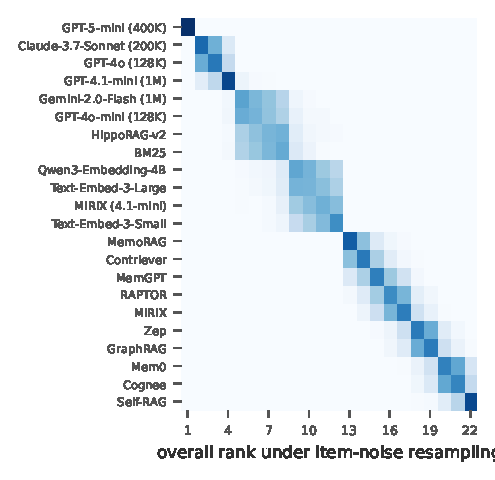
\includegraphics[width=0.6\linewidth]{figs/fig_ranks.pdf}
\caption{Probability of each overall rank for the 22 systems in MemoryAgentBench's main table under item
resampling (design effect 1). Rows are systems in their reported order.}
\label{fig:ranks}
\end{figure}
\section{Audited claims}
The full table of 268 comparisons, its verification sample and all scripts are released with the paper.
\end{document}
